%*****************************************
\chapter{La perception de l'environnement sonore}\label{ch:psycho_ea}
%*****************************************


Avant d'aller plus loin dans l'exposé de nos travaux, il nous semble indispensable de dresser ici un état des lieux des connaissances liées à la perception des sons. Nous procédons en cinq étapes. 

Dans la première, nous proposons un tableau général des différents processus intervenant dans le traitement de l'information sonore, processus mis en œuvre dès lors que le signal atteint le tympan. 

Dans la seconde, nous interrogeons la manière dont nous nous représentons le monde sonore perçu. Nous démontrons comment cette représentation influe sur notre perception. 

Dans la troisième, nous nous intéressons aux processus dits d'Analyse de Scènes Acoustiques (ASA), processus par lesquels le cerveau ségrègue les informations contenues dans l'environnement sonore afin d'en dégager des objets cohérents. 

Dans la quatrième, nous introduisons la notion de paysage sonore, et examinons l'impact que cette notion a sur les recherches en matière de perception des environnements. Nos travaux s'inscrivant largement dans cette approche, nous dressons un état de l'art des connaissances en matière de perception des paysages sonores, et tentons de dégager les grands axes méthodologiques suivis par ces études.

Enfin, dans la cinquième, nous nous attachons à définir les concepts d'événement et de texture sonore, notions clefs qui interviennent par la suite dans le modèle de scène sonore proposé.

\section{Le traitement de l'information auditive}

\subsection{Perception et cognition}

Perception. Le mot désigne l'ensemble des processus de traitement de l'information sensorielle. 
La perception du monde sonore qui nous entoure est un phénomène complexe, aujourd'hui encore mal connu. 

Cette perception est à l'origine de l'interaction que nous créons avec notre environnement. Elle détermine notre capacité d'adaptation à ce dernier. Cette relation au monde \emph{réel} ne se rompt jamais. Nous percevons des sons en permanence, et ce, même si aucune source sonore n'est présente. 

Ainsi tel mélomane dont la tête résonne encore de l'air, bien après que les instruments se soient tus. Ainsi tel usager des transports dont l'oreille anticipe (pour s'en protéger...) les crissements du métro alors que la rame n'est pas encore à quai.

Cognition. Selon U. Neisser\footnote{Ulric Neisser est considéré comme un des pères du cognitivisme notamment grâce à son livre \citep{neisser1967cognitive}. Il a par la suite critiqué la direction prise par le mouvement, dénonçant une "approche laboratoire" trop éloignée de la réalité terrain.} dans \citep[p. ??]{neisser1976cognition}:

\begin{quote}
``\,Cognition is the activity of knowing : the acquisition, organisation and use of knowledge.\,''
\end{quote}

Le mot désigne l'ensemble des processus d'acquisition et de développement d'une connaissance du monde. 

Selon la théorie classique, perception et cognition dépendent de deux groupes de systèmes fonctionnels du cerveau distincts. La perception mobilise les systèmes de traitement dits modaux, c'est à dire supportés par les organes sensoriels (oreilles, yeux etc $\ldots$), tandis que la cognition s'appuie sur des représentations mentales des réalités externes, par essence amodales.
 
Cette dichotomie entre perception et cognition est aujourd'hui remise en question. Dans une approche ``\,incarnée\,'' de la cognition (\emph{Grounded Cognition}), Barsalou nie le caractère amodal des représentations mentales prônant que ces dernières dépendent également des modalités sensorielles \citep{barsalou2010grounded}. Il tente ainsi de réunir les processus perceptifs et cognitifs \citep{goldstone1998reuniting, barsalou1999perceptions}.
Les deux approches sont illustrées sur la Figure~\ref{fig:processusPercepAndCo}.

\begin{figure}[bth]
        \myfloatalign
        \includegraphics[width=.8\linewidth]{gfx/Representation}
        \caption{Processus cognitifs et perceptifs}\label{fig:processusPercepAndCo}
\end{figure}

\subsubsection{Psychologie cognitive et psychoacoustique}

La psychologie cognitive est un domaine de recherche dédié aux phénomènes se rapportant à la connaissance. Elle est née dans les années 50, en réaction au \emph{Béhaviorisme}, théorie fondée sur ``\,l'étude des comportements objectivement observables de l'être humain\,'', et négligeant, de fait, le rôle de la conscience. La psychologie cognitive s'interroge sur des modèles théoriques complexes rendant compte de tous les faits et de toutes les lois connus. Les chercheurs y explorent tout à la fois, la mémoire, le langage, l'intelligence, la perception.
 
L'approche cognitiviste, dans le domaine de la perception auditive, se distingue de celle plus traditionnelle de la psychoacoustique \footnote{La psychoacoustique est une branche de la psychophysique qui applique au domaine de l'acoustique les concepts et les méthodes de la psychophysique}. Tandis que la psychoacoustique émet l'hypothèse d'une relation directe entre le stimulus et la réponse du sujet, la psychologie cognitive soutient que la réponse, elle, est entièrement corrélées au contexte, à l'expérience, aux interactions multi-sensorielles \citep{maffiolo_marieParis_1997}.

\gl{La réponse tient compte non seulement des traitements perceptifs mais aussi des représentations issues et de la mémoire individuelle (\ie~construites en particulier à partir de la relation sensible au monde) et de la mémoire collective, à travers le développement des connaissances partagées \citep[p. ??]{maffiolo_caracterisation_1999}.}

La psychologie cognitive s'intéresse prioritairement à l'aspect cognitif de la perception en considérant l'individu comme un tout. Elle prend en compte la culture, l'expérience, l'activité de l'individu et ne focalise pas seulement sur la réaction des organes sensoriels \gl{comme l'oreille}. Elle questionne les aspects qualitatifs plus que quantitatifs de notre compréhension du monde sonore \citep[p. ??]{maffiolo_caracterisation_1999}.

Elle envisage l'ensemble des étapes du traitement auditif de manière globale et permet ainsi de faire le lien entre une information sensorielle et une information abstraite \citep{mcadams1994penser}.

\gl{En psychologie cognitive, on distingue les approches cognitivistes, qui s'intéressent plus particulièrement aux processus montant (\emph{botttom-up}, \cf~section~\ref{sec:ch3_butd}) relatifs au traitement de l'information perçue, et les approches cognitives, qui interrogent, avant tout, les processus descendants (\emph{top-down}, \cf~section~\ref{sec:ch3_butd}) liés à la mémoire du sujet ainsi qu'au contexte \citep[p. ??]{guastavino_etude_2003}}.

\subsubsection{Paradigme de la psychologie cognitive}

Nous l'avons vu, \gl{la psychologie cognitive} ne conçoit pas le sujet comme une ``\,boîte noire\,'', mais reconnaît en lui un système de traitement de l'information. Il admet que l'individu adopte une stratégie afin d'optimiser le traitement des stimuli. Cette stratégie est déterminée par la nature du stimulus, mais aussi par son contexte, et par les connaissances a priori du sujet.

Maffiolo \citep[p. ??]{maffiolo_caracterisation_1999} propose une présentation des présupposés sur lesquels repose la psychologie cognitive (\Cf~Figure~\ref{fig:paradigmeCognitivisme}). Ces présupposés sont résumés ci-après:

\begin{itemize}
\item le monde est discrétisé en dimensions ou propriétés issues de la physique, et considérées comme vraies
\item ces dimensions ou propriétés peuvent être mesurées objectivement par des instruments. Elles rendent compte ainsi de la réalité
\item le sujet intègre de manière séquentielle ces dimensions ou propriétés en fonction du contexte
\item l'évaluation subjective du sujet est \gl{interprétée comme} un décalage par rapport à la mesure objective considérée comme vraie
\end{itemize}

Au regard du paradigme classique de la psychologie cognitive, Maffiolo met en évidence quatre points discutables :

\begin{itemize}
\item la pertinence des dimensions et propriétés physiques utilisées pour le découpage du monde
\item un traitement par les sujets tenant spécifiquement compte de ces dimensions
\item une séparation nette entre stimulus et contexte
\item le caractère subjectif du jugement humain en comparaison à l'objectivité d'un appareil de mesure.
\end{itemize}

\gl{commenter} \\

\begin{figure}[bth]
        \myfloatalign
        \includegraphics[width=\linewidth]{gfx/Shema_maffiolo}
        \caption[Paradigme de la psychologie cognititve]{Paradigme de la psychologie cognititve, d'après \citep{maffiolo_caracterisation_1999}}\label{fig:paradigme Cognitivisme}
\end{figure}

\subsection{L'approche Écologique}
\label{sec:ch3_ecologique}

L'approche écologique a d'abord été introduite dans le domaine de la vision par Gibson \citep{gibson1966senses}, qui se demande entre autre si les ``\,lois structurant les objets sont porteuses d'informations, ou si cette information est tirée de comparaisons \,'' \citep{gibson1978ecological}.

Cette approche reconnaît que la réponse à un stimulus dépend à la fois de l'information perçue, et de la connaissance du monde, autrement dit l'environnement quotidien et le contexte habituel d'écoute du stimulus.

\subsubsection{\emph{Soundwalk}}

Appliquée à la perception sonore, l'approche écologique requiert de prendre en compte l'environnement et du sujet, et du stimulus auquel il est exposé. La démarche s'oppose aux méthodes expérimentales traditionnelles, celle(s) de la psychophysique en particulier, sur le postulat que les expériences en laboratoire décontextualisent le sujet et sa réponse. Une expérience en laboratoire demande en effet au sujet de fournir un effort d'abstraction supplémentaire afin de s’imaginer dans des conditions d'écoute réelle.

Nombre d'études désormais sont réalisées dans un cadre \emph{in situ}. On parle d'ailleurs de \emph{soundwalk}  \footnote{\emph{Soundwalk} est un terme anglais introduit par R. Murray Schafer \citep{schafer1969new} signifiant littéralement ``\,marche sonore\,''. Ce terme étant couramment utilisé en français, il ne sera pas traduit dans ce document} pour désigner les expériences où le sujet est immergé dans l'environnement qu'il doit évaluer \citep{adams2008soundwalking,jeon2013soundwalk}.


La méthode des \emph{soundwalk} permet entre autre:

\begin{itemize}
\item  de contextualiser le sujet, à savoir, l'évaluer dans un environnement qu'il connaît (lieu de vie, de travail)
\item d'évaluer l'environnement sonore, tout en maintenant actif les autres sens (vue, olfaction)
\item d'éluder le problème de la reproduction des environnements sonores en laboratoire
\end{itemize}

Malgré tout, les études \emph{in situ}, bien que valides écologiquement, présentent elles aussi des inconvénients. Dans l'hypothèse où tous les sujets ne passent pas l'expérience en même temps, il est impossible de garantir à chacun les mêmes stimuli et/ou le même environnement. Se pose le problème de la reproductibilité des expériences. Inversement, dans l'hypothèse où tous les sujets passent l'expérience en même temps, il peut se poser des problèmes d'organisation de nature à compromettre une égale réceptivité, disponibilité chez tous les sujets.

\subsubsection{Reproduction écologique des environnements sonores en laboratoire}

Le problème de la reproduction écologique des environnements sonores en laboratoire a été particulièrement étudié par Guastavino. \citep{guastavino2003approche,guastavino2004perceptual,guastavino2005ecological}. En comparant les descriptions verbales produites à la suite d'écoutes \emph{in situ} , et d'écoutes en laboratoire, via des systèmes de reproduction stéréophoniques et multi-phoniques, \citep{guastavino2005ecological} montre que les événements sonores peuplant les scènes sont décrits de la même manière, quel que soit le contexte d'écoute.

Cependant des différences apparaissent au niveau de la description des fonds sonores (\emph{backgrounds}), entre les écoutes stéréophoniques, et les écoutes multi-phoniques et \emph{in situ}, suggérant de fait que le système de reproduction influe sur les processus cognitifs mis en œuvre. Des conclusions similaires sont faites dans \citep{guastavino2004perceptual} s'agissant cette fois de systèmes de reproduction mono, stéréo, et multi-phoniques.

\gl{selection des stimuli} \\

\subsection{Le chaîne traitement de l'information auditive}
\label{sec:chaineTaite}

Le son est une vibration émise par une source d'excitation, et transmise à l'air. Cette vibration se propage ensuite jusqu'à atteindre un récepteur, le tympan, qui va capter le différentiel de pression résultant de cette vibration. C'est le point de départ du processus de traitement de l'information auditive. 

Si on adopte une approche \emph{traitement de l'information}, on peut décomposer ce processus en plusieurs systèmes inter-connectés. Ces systèmes forment une chaîne qui, au fur et à mesure des traitements, interprète le signal acoustique afin d'en extraire l'information sémantique. Plus on se place loin dans la chaîne de traitement, plus on a accès à une information abstraite, potentiellement utilisable par d'autres processus de haut niveau. La figure \ref{fig:traitementSonMcAdamsBigand} extraite de \citep{mcadams1994penser} nous donne un aperçu des principales fonctionnalités du système de traitement auditif.

\begin{figure}[t]
        \myfloatalign
        
\includegraphics[width=.6\linewidth]{gfx/traitementSonMcAdamsBigand}
        \caption[Principaux processus de traitement de l'information auditive et leurs interactions]{Principaux processus de traitement de l'information auditive et leurs interactions, d'après \citep{mcadams1994penser}}\label{fig:traitementSonMcAdamsBigand}
\end{figure}

Lors de l'étape de \emph{transduction}, les vibrations sonores parvenant au tympan sont analysées puis traduites en impulsions nerveuses transmises au cerveau. Ces impulsions rendent compte des attributs spectraux et temporels de l'onde. L'extraction des composantes fréquentielles intervient dans la cochlée. C'est à l'intérieur de cette dernière que les différentes parties de la membrane basilaire vont être excitées en fonction des fréquences composant le signal, suivant un axe tonotopique. Les vibrations captées à chaque point d’excitation de la membrane basilaire sont transmises au cerveau via les nerfs auditifs, chaque point codant une information correspondant à une bande fréquentielle limitée. 

Vient ensuite le \emph{processus de groupement auditif}. C'est une étape d'intégration temporelle au cours de laquelle l'information est analysée en images auditives cohérentes. Contrairement à ce que pensaient les Grecs, nous ne possédons pas de "canaux" séparés pour chaque objet sonore présent dans l'environnement \citep{yost1994fundamentals}. C'est notre cerveau qui se charge de fusionner et de discrétiser les éléments sonores simultanés afin de créer un flux auditif structuré. En d'autres termes, il détermine le nombre d'objets présents, identifie leur provenance, et en définit le sens. 

Afin d'illustrer notre propos, mettons nous dans la peau du mélomane écoutant cette fois un Choral de Bach. C'est le \emph{processus de groupement auditif} qui nous permet, sur la base des paramètres spectro-temporels du signal, de distinguer les quatre voix basse, ténor, alto et soprano. Par contre c'est à partir d'une analyse des attributs perceptifs que nous sommes capables de percevoir les mélodies comme des objets unitaires, même si ces dernières sont développées entre les différentes voix du choral. Cette extraction des propriétés perceptives intervient pendant la phase dite \emph{d'extraction/calcul des propriétés/attributs}.

Les travaux menés au titre de l'Analyse de Scènes Auditives (ASA) dont le sujet est abordé plus bas (\Cf~section~\ref{sec:ch3_ASA}), ont largement porté sur ces processus de groupement.

\subsection{Processus \emph{Bottum-up} et processus \emph{Top-down}}
\label{sec:ch3_butd}

L'interaction entre l'homme et son environnement est fonction d'une part de l'information sensorielle captée par le sujet, d'autre part de la rétroaction exercée par lui sur ces données. Cette rétroaction est déterminée par son expérience sensible du monde. Par "expérience sensible", nous entendons la mémoire interne des interactions passées, mémoire grâce à laquelle nous optimisons l'analyse des stimuli, et intégrons les effets de contexte dus à l'environnement.

Cette mémoire est à la fois :

\begin{itemize}
\item individuelle : dépendant de notre expérience propre
\item collective : dépendant des connaissances que nous avons acquises sur le monde
\end{itemize}

La rétroaction est l'expression de l'individualité du sujet, individualité qui explique que deux personnes, ayant des capacités sensorielles semblables, peuvent percevoir différemment un même environnement.

Ainsi la perception mobilise deux formes de traitements :

\begin{itemize}
\item les traitements dits ascendants (bottom-up) dirigés par les données
\item les traitements dits descendants (top-down) dirigés par les concepts ou les représentations
\end{itemize}

Étudier la perception demande de prendre en compte aussi bien l'information externe (processus ascendant) que l'information interne (processus descendant). Réduire la perception à une simple association de sensations ne permet pas de rendre compte de l'éventail des processus cognitifs entrant dans le décodage de l'environnement. Un exemple concret, emprunté au domaine de la vision, est celui du phénomène dit de bi-stabilité, \ie~La faculté, chez un sujet, de tirer d'un même stimulus deux analyses différentes, mais jamais simultanément (\Cf~Figure~\ref{fig:bistabilite}). \\

\begin{figure}[bth]
        \myfloatalign
        \includegraphics[width=.6\linewidth]{gfx/canard_lapin}
        \caption[Le phénomène de bistabilité: l'illusion du canard-lapin]{Le phénomène de bistabilité: l'illusion du canard-lapin. Première publication dans \emph{Fliegende Blätter}, 23 octobre 1892, p. 147}\label{fig:bistabilite}
\end{figure}

\gl{ajout: \citep{schwartz2012multistability}}\\

Un autre exemple, cette fois dans le domaine de l'audition, nous semble illustrer le caractère dual de la perception. Il est donné par McAdams et Bigand \citep[p. 2]{mcadams1994penser}:

\begin{quote}
``\,...Imaginez vous un instant en pleine forêt amazonienne : vous entendriez exactement les mêmes bruits que le guide qui vous accompagne, mais, étant donné votre manque de connaissance du milieu, vous seriez incapable d'extraire du fond sonore les sons correspondant aux cris de l'iguane, aux singes macaques, aux chants des ouistitis ou aux bruissements des arbres tropicaux. De ce fait vous seriez dans l'incapacité d'attribuer une signification à l'ensemble de la structure sonore, ce qui pourrait être important pour votre survie dans l'environnement.\,''
\end{quote}

\subsection{L'écoute}

\section{Représentation mentale de l'environnement sonore}

Le cerveau entretien un dialogue constant avec l'environnement sonore. Ce dialogue s'effectue par le biais des représentations mentales. Une définition des représentations mentales est donnée par \citep{houde1998vocabulaire}:

\begin{quote}
``\,La représentation mentale peut être vue comme une entité interne, le correspondant cognitif individuel des réalités externes expérimentées par un sujet.\,''
\end{quote}

Ces représentations font office de sauvegardes de l'information. Conservées en mémoire sous une forme hautement abstraite \citep[p. ??]{mcadams1994penser}, elles rendent compte à la fois de notre compréhension du monde et de la manière dont nous l'abordons. Ces connaissances subjectives, non directement observables, restent néanmoins accessibles au chercheur par le biais d'expériences d'objectivation (voir section~\ref{sec:appCategorielle})
 
Ces représentations forment une image mentale discrète d'un monde réel continu \citep{houde1998vocabulaire}. C'est par le passage du continu au discret que nous sommes à même d'organiser nos connaissances, afin de les réutiliser de manière efficace. Les objets discrets issus de cette organisation sont appelés des catégories. L'action consistant à juger si un événement perçu appartient à une catégorie, est appelée la catégorisation.

\subsection{La notion de catégorie}

\subsubsection{Définition}

\gl{Généralité sur la catégorisation} \\

Une des vérités de tout être humain est de segmenter son environnement, \ie~de se bâtir un système de classification permettant de regrouper des objets n'étant pas identiques \citep[p. 1]{rosch1978cognition}. On appelle catégorisation, l'action consistant à regrouper des objets du monde physique considérés comme équivalents, et catégorie, l'entité mentale contenant le groupe d'objets ainsi rassemblés. 
 
D'un point de vue écologique, la catégorisation est un processus essentiel. Nous sommes constamment en train de catégoriser l'environnement, et devons être à même, à tout moment, de prendre une décision sur l'appartenance catégorielle d'un objet. Ce processus est adaptatif. La prise de décision est toujours fonction du sujet, d'une situation et d'un contexte. Ainsi, un même objet, perçu à deux moments distincts, pourra être affecté à des catégories différentes. \\

\gl{La nature des catégories} \\

\subsubsection{Utilité des catégories}

Avant de parler de l'utilité des catégories, voyons où et comment s'exerce les catégorisations dans notre quotidien. \citep{anderson1991adaptive} identifie trois occurrences: \\

\begin{itemize}

\item Le langage est le lieu, par excellence, des catégories. Catégoriser, c'est considérer un objet comme un élément distinct du monde. Cette distinction s'accompagne généralement (pas toujours) d'une désignation. C'est l'essence même des processus d'identification que de chercher à nommer les objets, une fois qu'ils ont été isolés. Il est raisonnable de penser que, de la même manière, une catégorie possède un label associé. On parlera alors de catégorie(s) sémantique(s). Cette relation entre langage et catégorie nourrit le débat sur l'universalité présupposée de la catégorisation. L'opération permanente consistant à isoler un objet, et à lui attribuer un nom, est l'antinomie du ``\,geste adamique\,'', \ie~d'attribution libre du nom, hors toute influence et/ou contexte (d'Adam, le premier homme révélé et nommé dans la bible). La langue est un code partagé par une communauté. Dans une certaine mesure, sa définition, \ie~le sens donné aux mots, peut varier suivant les groupes de cette communauté. Ainsi, catégoriser ne dépend pas seulement d'une réalité physique du monde, mais également d'un contexte socioculturel. La catégorisation peut être vue comme une action intermédiaire entre, d'une part, l'organisation d'une connaissance individuelle résultant d'une expérience sensorielle personnelle, et, d'autre part, la constitution d'une représentation collective pouvant être partagée par le biais d'un langage commun \citep{dubois2006cognitive}.
\item le regroupement par similarité des caractéristiques: Nous sommes capables de regrouper des objets possédant des caractéristiques similaires, et ce, même si ces objets nous sont inconnus \citep{fried1984induction}.
\item le regroupement par similarité fonctionnelle: Nous sommes capables d'interpréter des objets possédant des fonctions similaires comme faisant partie d'un même groupe, et ce même si ces objets ont des caractéristiques distinctes. Pour exemple: deux hommes descendant d'un camion de pompier pour éteindre un feu de forêt seront catégorisées comme des pompiers, ce indépendamment des tenues qu'ils portent. Quand nous parlons de la catégorisation comme du processus de discrétisation du monde réel, ce "monde réel" englobe et la réalité des faits physiques, et la réalité des faits sociologiques.
\end{itemize}



\gl{Quel est l'effet de la catégorisation} \\

\subsection{Le processus de catégorisation}

La catégorisation est nécessairement un outil supervisé, \ie~nous ne pouvons catégoriser les objets qu'à partir des catégories que nous connaissons. Le processus catégoriel procède suivant deux mécanismes:
\begin{itemize}
\item mécanisme inductif: associer un objet à une catégorie sur la base des caractéristiques perçues de ce dernier
\item mécanisme déductif: associer à un objet les caractéristiques de la catégorie à laquelle il appartient
\end{itemize}

\subsubsection{Capacité d'inférence}

\subsection{Organisation de la structure catégorielle}

Le cerveau doit en permanence faire sens d'une information riche et variée, et ce de manière productive. Afin de satisfaire à cette exigence d'efficacité, l'organisation catégorielle doit répondre à deux grand principes \citep[p. 29]{rosch1978cognition}:

\begin{itemize}
\item L'économie cognitive
\item La redondance structurelle
\end{itemize}

\subsubsection{L'économie cognitive}

La catégorisation doit fournir un maximum d'informations pour un minimum d'effort. C'est pourquoi la logique catégorielle prend en compte le contexte sensoriel. En résumé, le traitement de l'objet s'opère et par rapport à lui, et par rapport au traitement des objets perçus et catégorisés simultanément. Comme énoncé par D. Dubois \citep[p. 33]{dubois1991semantique}:

\begin{quote}
``\,Catégoriser un stimulus signifie le considérer dans la finalité de cette catégorisation, non seulement comme équivalent des autres stimuli de la même catégorie, mais également différent des stimuli qui n'appartiennent pas à cette catégorie\,''.
\end{quote}

Du principe d'économie cognitive, il découle que la catégorisation de l'objet n'est pas une catégorisation dans l'absolu. Elle ne dépend pas uniquement de l'observation des propriétés particulières de l'objet, mais également du contexte dans lequel il est appréhendé.

\subsubsection{La redondance structurelle}

L'ensemble des objets physiques ne vit pas dans un espace fini, identifié, et dont les valeurs seraient équiprobables. Le monde ne se résout pas à des paramètres dimensionnés, indépendants et manipulables, comme dans le cadre d'études en laboratoire. Au contraire. Il peut exister des discontinuités saillantes entres objets, de même que ces objets peuvent être liés entre eux par des patterns de co-occurrence de propriétés (exemple : un chien possède "quatre pattes et un museau" plus souvent que "deux pattes et un museau"). Ces discontinuités et corrélations, présentes dans les propriétés perçues, étayent la structure catégorielle de notre représentation mentale, et gouvernent ainsi le processus de catégorisation.
 
\subsubsection{Catégorie et abstraction}
 \label{sec:ch3_categoEtAbstract}
 
Rosch propose de voir la structure catégorielle suivant deux axes \citep[p. 30-41]{rosch1978cognition}:

\begin{itemize}
\item \textit{axe vertical}: L'axe vertical fixe l'organisation hiérarchique des catégories, et permet d'appréhender l'imbrication de ces catégories les unes par rapport aux autres. \gl{Ce faisant, il en dresse la taxonomie}, les catégories de haut-niveaux représentant des objets abstraits ou concepts, et incluant un grand nombre de sous catégories, et les catégories de bas-niveaux représentant des objets concrets, incluant peu de sous catégories. Ainsi, plus le niveau d'abstraction est grand, plus les similitudes entre objets d'une même catégorie (intra-catégorielle), ainsi que les similitudes entre objets de catégories distinctes (inter-catégorielle) son faibles. Inversement, plus le niveau d'abstraction est faible, plus les similitudes intra- et inter-catégorielles sont élevées. Rosch propose de décomposer cette dimension verticale en trois niveaux d'abstraction (\Cf~Figure~\ref{fig:categorieLVL}): Superordonné, Base et subordonné. Le niveau superordonné regroupe les catégories à haut niveau d'abstraction. Les périmètres de ces catégories sont larges (Mobilier, Véhicule...) \ie~les objets qu'elles contiennent peuvent être très distincts. Le niveau subordonné regroupe les catégories à bas niveau d'abstraction, ou catégories concrètes. Les périmètres de ces catégories sont plus précis (Chaise longue, Cabriolet...), et les objets qu'elles contiennent sont nécessairement très similaires. On notera ici que les objets de la classe Cabriolet présentent plus de propriétés communes avec les objets de la classe Berline (c'est un exemple...), que n'en sauraient partager les objets des classes Mobilier et Véhicule.
\item \textit{axe horizontal}: L'axe horizontal fixe, lui, l'organisation ``\,géographique\,'' des catégories, et permet d'appréhender, d'une part, les périmètres de ces catégories au sein d'un même niveau d'abstraction, d'autre part, la typicité des objets contenus dans une même classe. Bien sûr, les catégories ne sont pas des objets strictement discrets, et les propriétés des objets qu'elles regroupent peuvent se trouver attribuées à d'autres objets, dans d'autres catégories. Ainsi, les frontières entre les différentes catégories ne sont pas figées, et peuvent même se recouvrir.
\end{itemize}

\begin{figure}[bth]
        \myfloatalign
        \includegraphics[width=.6\linewidth]{gfx/categorieLVL}
        \caption{Les trois niveaux d'abstraction de l'axe vertical de la structure catégorielle.}\label{fig:categorieLVL}
\end{figure}

\subsection{Théories de la catégorisation}

\gl{\citep{goldstone2003concepts}}

\subsubsection{Théorie classique}

\subsubsection{Théorie prototypique}

Nous traitons ici du processus de catégorisation formalisé par E. Rosch et B. B. Lloyd \citep{rosch1978cognition}, et nommé théorie prototypique de la catégorisation.
 
Pour discriminer les catégories, Rosch propose de ne pas raisonner en terme de frontières, mais plutôt de décrire chaque catégorie par un nombre de cas non ambiguës (clear case) \citep[p. 36]{rosch1978cognition}. Tous les objets d'une catégorie ne sont pas également représentatifs de cette dernière, les cas non ambiguës peuvent être vus comme les objets les plus typiques de la catégorie. Ce fait est empirique, il a été montré que des sujets peuvent très bien s'accorder sur la typicité d'un objet par rapport à une catégorie, tout en n'étant pas d'accord sur les frontières de cette dernière \citep{rosch1974human,rosch1975cognitive}. Le terme prototype, qui donne son nom à la théorie, vient de l'assertion que, parmi ces cas non ambiguës, il en existe un, le prototype, plus représentatif que les autres, et qui forme le noyau de la catégorie.

Les catégories sont structurées en interne, en référence à un prototype, \ie~l'objet possédant les attributs typiques de celle-ci. L'appartenance d'un objet à une catégorie dépend alors de la ressemblance qu'entretient ce dernier avec le prototype.  Plusieurs propositions ont été faites afin de définir le prototype d'une catégorie: Pour Tversky \citep{tversky1977features}, l'élément prototype est celui dont la somme des similarités avec les autres éléments de la catégorie est la plus élevée. Pour \citep{rosch1975family}, il s'agit de l'objet possédant le plus de propriétés en commun avec les objets de la catégorie, et le moins de propriétés avec les objets des catégories externes. La typicité d'un élément d'une catégorie s'évalue à la fois en fonction de son degré d'appartenance à celle-ci, et de son degré de différenciation vis à vis des autres catégories. 

\gl{En se limitant à l'observation d'attributs vivant dans un espace métrique, \citep{reed1972pattern, rosch1976structural} ont montré que le prototype est un centroid, un objet défini comme étant la moyenne des attributs des objets de la catégories.}

Mais il faut bien comprendre que cette théorie prototypique de la catégorisation, bien que se basant sur des faits expérimentaux, est avant tout une vision pratique, un concept qui n'a pas été clairement défini et dont l'implication dans les processus de catégorisation reste floue \citep[p. 36-40]{rosch1978cognition} \citep[p. 49-54]{dubois1991semantique}.

\subsubsection{Théorie de l'exemplaire}

La théories des exemplaires ou \textit{context theory} \citep{medin1978context}, et son extension multidimensionnelle \citep{medin1978context}

\subsubsection{Autres théories}

\subsection{Similarité et catégorisation}

\subsection{Catégorisation et contexte sensoriel}
\label{sec:ch3_identification et Contexte}

G1: \citep{ballas1987interpreting,niessen2008disambiguating,gygi2011incongruency} \\


\section{Analyse de scènes acoustiques}
\label{sec:ch3_ASA}

\subsection{Définition}
\label{sec:ASAintro}

L'analyse de scène(s) est d'abord apparue dans le domaine des recherches informatiques en vision. Le terme fait référence aux différentes stratégies par lesquelles un ordinateur parvient à isoler un objet d'une image~\citep[p. 12]{mcadams1994penser}. Le pendant \gl{perceptif et auditif} de l'analyse de scènes est l'Analyse de Scène(s) Acoustique(s). L'ASA a été introduite par A. S. Bregman dans son ouvrage de référence\citep{bregman1994auditory}.

L'ASA désigne l'ensemble des traitements perceptifs permettant d'isoler, dans une mixture sonore, les informations émanant de sources distinctes, et de les "organiser" en un tout cohérent. Ces regroupements sont nécessaires au cerveau, et donc au sujet, pour comprendre, pour donner sens à l'environnement. On parle de processus de ségrégation ou de processus de groupement \citep{winkler2009modeling}. Comme vu précédemment section~\ref{sec:chaineTaite}, ces processus mobilisent à la fois les traitements ascendants ou bottom-up, intervenant au niveau de l'information auditive transduite, et les traitements descendants ou top-down, intervenant au niveau du bagage mémoriel. Les processus \emph{bottum-up} sont appelés \emph{processus primitifs}, et les processus  \emph{top-down}, \emph{processus basés sur des schémas}. 

Les \emph{processus primitifs} sont innés, et opèrent à partir des régularités du signal, afin d'en regrouper les composantes fréquentielles produites par une même source. Le mot régularité désigne ici les propriétés constantes de l'environnement, perçues par tous les hommes, et en tous lieux. Par exemple, si la fréquence fondamentale d'un son harmonique change au cours du temps, toutes ses harmoniques changeront également afin de maintenir la structure harmonique du son [p. 38]\citep{bregman1994auditory}.

Les \emph{processus basés sur des schémas} sont eux conditionnés, et opèrent sur la base de connaissances, ou schémas, partie intégrante de notre représentation mentale du monde, représentation construite sur la base des écoutes antérieures. 
 
\subsection{Une approche psychoacoustique}

\gl{Si la plupart des recherches sur l'ASA adoptent une approche cognitive, se concentrant sur l'étude des \emph{processus primitifs}}, elles suivent généralement une méthodologie expérimentale très inspirée de la psychoacoustique. De fait, les sujets sont soumis à des stimuli décrits analytiquement dans un espace multidimensionnel de dimensions physiques (fréquence, intensité etc $\ldots$) \citep{dubois2006cognitive}. Dans la majorité des cas, ces stimuli ou sons, qu'ils soient purs ou qu'ils soient complexes,\footnote{Un son pur est un son composé d'une seule sinusoïde, \ie~possédant une seule fréquence. Un son complexe est, lui, composé de plusieurs composantes fréquentielles} sont synthétisés en laboratoire.

Ces sons sont proposés à l'écoute de manière séquentielle. Au cours de l'expérience, les paramètres en sont modifiés (intensité, hauteur fréquentielle, espace entre les séquences...) afin d'évaluer le seuil à partir duquel la capacité du sujet de distinguer les sources sonores sont altérées.

L'étude de l'ASA se borne donc à l'analyse de l'effet de descripteurs "bas niveau" dans le(s) processus d'intégration(s), sans tenir compte d'attributs perceptifs "haut niveau", comme la valeur sémantique attribuée aux sons, sans tenir compte non plus de considérations écologiques~\ref{sec:ecologique}. C'est pourquoi il est difficile de faire le lien entre la notion de source sonore ayant cours dans le domaine de la psychoacoustique, et celle admise dans le domaine de la psychologie cognitive. En théorie, dans l'une et l'autre approche, le terme source sonore se réfère à l'objet (\eg~voiture) supposé en être la source. Mais, en psychologie cognitive, cette relation est naturelle, le stimulus étant le plus souvent un enregistrement de ladite source, tandis qu'en psychoacoustique cette relation est dénaturée, le stimulus, synthétisé, étant un objet abstrait (agglomérat de sinusoïdes) dont l'existence n'est avérée que dans la mesure où il est interprété par le sujet comme un tout, une entité. Les résultats, obtenus à partir de tels stimuli, éloignés de la réalité des phénomènes acoustiques perçus, sont difficiles à généraliser à des applications plus incarnées. Nous touchons là aux limites de l'approche psychoacoustique appliquées aux études des \emph{processus primitifs} de l'ASA. \gl{Les résultats, obtenus à partir de stimuli très éloignés de la réalité des phénomènes acoustiques perçus, étant difficiles à généraliser à des applications plus incarnés.}

\subsection{Régularités et processus primitifs}

L'existence des \emph{processus primitifs} est une conséquence de l'efficience, dans le monde sonore, de régularités universelles affectant l'ensemble des stimuli auditifs. Bregman distingue 4 types de régularités [p. 19,21,31,33]\citep{mcadams1994penser}:

\begin{enumerate}
\item \emph{Synchronicité}: Il est rare que des sons n'ayant aucun rapport entre eux démarrent et s'arrêtent au même moment.
\item \emph{Continuité}: 
\begin{itemize}
\item Les propriétés d'un son isolé tendent à se modifier lentement et de façon continue.
\item Les propriétés d'une séquence de sons émis par la même source tendent à se modifier lentement.
\end{itemize}
\item \emph{Harmonicité}: Lorsqu'un corps sonore vibre à une période répétée, ses vibrations donnent naissance à un pattern acoustique dont les fréquences des composants sont des multiples d'une même fréquence fondamentale
\item \emph{Uniformité}: La plupart des modifications qui surviennent dans un signal acoustique affectent tous les composants du son résultant, de manière identique et simultanée.
\end{enumerate}

Notre perception du monde est assujettie à ces lois. 
Les \emph{processus primitifs}, sensibles aux stimuli exclusivement, nous permettent d'isoler du monde sonore des objets cohérents perçus à travers le prisme desdites régularités\citep{ballas1987interpreting}. Le fait est qu'un principe similaire de perception des formes s'applique également au domaine de la vision.

\subsection{Perception de la forme}

Que ce soit en vision ou en audition, notre cerveau est en permanence stimulé par une multitude de sources distinctes. Percevoir un objet dans cet agglomérat, c'est être capable d'isoler tous les signaux émis par une même source, et de les réunir en une unité perceptive cohérente.

Parmi les premiers travaux qui se sont intéressés à ces processus de groupement, on trouve la psychologie de la forme, en allemand \emph{Gestalt Theory}. Cette théorie, introduite par Ernst Mach et Christian von Ehrenfels à la fin du XIXème siècle, se propose d'expliciter les principes selon lesquels des stimuli sensoriels sont combinés afin de former un pattern mental rendant compte de la présence d'un objet présent dans l'environnement.

Mis en évidence en perception visuelle, ces principes restent vrais en perception auditive\citep[ch. 1]{bregman1994auditory}. Parmi ces principes, nous en détaillons ici cinq:

\begin{enumerate}
\item \emph{Proximité}: Des éléments proches les uns des autres ont tendance à être groupés ensemble. En audition, ce principe de proximité opère suivant les différentes caractéristiques du son, à savoir, la fréquence, l'\emph{onset} \footnote{En traitement du signal audio, on désigne par le mot anglais \emph{onset} le début du signal. Ce terme étant couramment utilisé en français, nous ne le traduirons pas dans ce document.} et l'intensité.
 
\item \emph{Similarité}: Des éléments qui se ressemblent ont tendance à être groupés ensemble. 

Dans le domaine de la vision, la proximité est une notion de spatialité. La similarité, elle, s'applique aux caractéristiques physiques de l'objet (forme, couleur, etc $\ldots$), qui ne peuvent se décrire dans une dimension unique. 

Dans le domaine de l'audition, la proximité est généralement admise comme notion de temporalité (\emph{onsets} proches). Pour le reste des descripteurs, il est cependant difficile de distinguer les principes de proximité et de similarité. Bregman propose de parler proximité lorsqu'on traite d'une dimension physique particulière, et de parler similarité dès lors qu'on considère un ensemble de descripteurs, ou lorsque l'on traite d'attributs qui ne peuvent être clairement décomposés suivant des dimensions distinctes, comme le timbre.

\item \emph{Continuité}: Des éléments qui varient de manière non abrupte ont tendance à être groupés ensemble. Par ce principe, des objets distincts mais proches temporellement \gl{(respectivement spatialement pour la vision)} ont tendance à être perçus comme le prolongement des uns par rapport aux autres. A contrario, une changement abrupte indique généralement l'apparition d'une nouvelle source. C'est ce principe qui nous permet de percevoir comme une seule entité, un objet dont les caractéristiques varient dans le temps,\eg~le son d'une sirène.

De récentes études en neurosciences ont montré l'importance de ce principe dans les processus de groupement. Notamment \citep{winkler2009modeling} qui propose de voir l'ASA comme un processus prédictif, le cerveau cherchant à anticiper la nature des stimuli qui lui parviennent, sur la base de régularités extraites des objets détectés dans l'instant précédant.

\item \emph{Clôture}: Des éléments discontinus qui suggèrent la forme d'un objet continu ont tendance à être groupés ensemble. De manière automatique, le cerveau tend à percevoir un ensemble d'objets distincts comme un tout. En audition, ce principe est très lié à la notion de masquage. En effet, les sons que nous percevons sont régulièrement masqués par d'autres sons concurrents, éventuellement plus forts. Le principe de clôture nous permet de compenser ce phénomène de masquage et de percevoir le signal sans discontinuité. Ainsi lorsqu'un son pur est régulièrement entrecoupé de silences, nous percevons une série de sons purs, mais, si ces silences sont comblés par un bruit blanc, nous percevons un son pur continu. Ce phénomène est parfois appelé ``\,l’illusion de continuité\,'' \citep{dannenbring1976perceived}, et s'applique particulièrement dans le contexte de la perception de la parole \citep{carlyon2002continuity}.

\item \emph{Destin commun}: Des éléments qui varient de manière synchrone et uniforme ont tendance à être groupés ensemble. Comme évoqué à la section~\ref{sec:ASAintro} c'est ce principe qui permet de percevoir comme un tout les différentes harmoniques qui composent un son complexe. C'est également ce principe qui nous incite à percevoir de manière unie des stimuli ayant le même \emph{onset} temporel.
\end{enumerate}

Ces principes agissent de concert afin de grouper les composantes du son en flux auditifs.

\subsection{Flux auditif et stratégie de groupement}

\begin{figure}[bth]
        \myfloatalign
        \subfloat[]
        {\includegraphics[width=.5\linewidth]{gfx/tonesim_slow-eps-converted-to}}
        \subfloat[]
        {\includegraphics[width=.5\linewidth]{gfx/tonesim_fast-eps-converted-to}}
        \caption[Groupement séquentiel : proximité temporelle.]{Groupement séquentiel: proximité temporelle. Dans l'exemple (a), la durée entre les événements est telle qu'aucun groupement n'est effectué, les sons sont perçus comme des événements distincts. Dans l'exmple (b) la durée entre les événements est réduite, et un groupement s'opère suivant la proximité fréquentielle. Deux flux sont ainsi créés, le premier (rouge) regroupe les sons haute fréquence, et le deuxième (vert) les sons basse fréquence.}\label{fig:tonesim}
\end{figure}

\begin{figure}[bth]
        \myfloatalign
        \subfloat[]
        {\includegraphics[width=.5\linewidth]{gfx/gallop_2flux-eps-converted-to}}
        \subfloat[]
        {\includegraphics[width=.5\linewidth]{gfx/gallop_1flux-eps-converted-to}}
        \caption[Groupement séquentiel : proximité fréquentielle.]{Groupement séquentielle: la proximité fréquentielle. Deux groupes de sons sont joués à deux fréquences. Dans l'exemple (a), la distance entre les fréquences des sons est telle que deux flux sont créés, le premier (rouge) regroupe les sons haute fréquence, et le deuxième (vert) les sons basse fréquence. Dans l'exemple (b) la distance entre les fréquences est réduite et un groupement s'opère suivant la proximité fréquentielle. Un seul flux est créé, et l'on perçoit un pattern temporel rappelant le galop d'un cheval.}\label{fig:galop}
\end{figure}

\begin{figure}[bth]
        \myfloatalign
        \includegraphics[width=.5\linewidth]{gfx/harmo-eps-converted-to}
        \caption[Groupement simultané : régularité harmonique]{Groupement simultané : régularité harmonique. Un son complexe est joué plusieurs fois. A chaque occurence, on abaisse les hauteurs de la fréquence fondamentale et des harmoniques de manière uniforme. Une harmonique est conservée à fréquence constante (trait gras). Au début, un flux est créé, \ie~les harmoniques et la fréquence fondamentale sont perçus comme étant un seul objet. Au fur et à mesure que la régularité harmonique est brisée, le cerveau tend à percevoir l'harmonique à fréquence constante dans un flux séparé, \ie~comme étant un second objet.}\label{fig:harmo}
\end{figure}

\begin{figure}[bth]
        \myfloatalign
        \subfloat[]
        {\includegraphics[width=.5\linewidth]{gfx/opn1-eps-converted-to}}
        \subfloat[]
        {\includegraphics[width=.5\linewidth]{gfx/opn2-eps-converted-to}}
        \caption[Groupement ancien-plus-nouveau]{Groupement ancien-plus-nouveau. Dans l'exemple (a), les sons A et B ont des fréquences éloignées. Le cerveau génère deux flux, le premier relatif au son A (rouge), et le deuxième comprenant les sons B et C (vert). Dans l'exemple (b), les sons A et B ont la même fréquence. Le cerveau interprète le son B comme étant une continuité du son A. L'attraction entre B et C en est réduite. Le cerveau génère toujours deux flux, le premier regoupant cette fois ci les sons A et B (rouge), et le deuxième le son C (vert).}\label{fig:oldplusnew}
\end{figure}

L'une des notions les plus importantes en ASA est le concept de flux auditif (\emph{auditory stream}), que Bregman définit comme ``\,le groupement perceptif que nous faisons des parties du spectre qui vont ensemble\,''.

Contrairement au terme ``\,son\,'', qui peut faire référence aux réalités physiques des phénomènes acoustiques, aussi bien qu'aux représentations mentales que nous nous en faisons, le flux auditif désigne spécifiquement une entité perceptive.

Le terme flux se veut volontairement généraliste. Ce dernier peut désigner aussi bien un son isolé (un coup de marteau), comme plusieurs sons à condition que ces derniers soient perçus comme formant une seule entité (une série rapprochée de coups de marteau).

On désigne par ``\,formation de flux auditive\,'' (\emph{auditory streaming}) , le processus à l'origine de la création de flux. \citep{winkler2009modeling} propose la définition suivante en ce qui concerne la formation de flux auditifs:

\begin{quote}
``\, Un phénomène perceptif dans lequel une séquence de sons est perçue comme étant composée de deux ou plusieurs flux auditifs \,''
\end{quote}

Comme nous venons de le voir, le flux désigne une représentation perceptive d'un son, et, à ce titre, il est l'équivalent auditif de l'objet pour la vision \citep[p. 11]{bregman1994auditory}. Cependant, nous notons que la notion de flux, et plus particulièrement celle de formation de flux, est souvent utilisée dans un contexte où une dimension temporelle est sollicitée. On parle d'ailleurs de construction de flux  (\emph{build-up of streaming}) pour désigner la période durant laquelle le cerveau accumule des indices afin de générer et stabiliser les flux auditifs  \citep{cusack2004effects,snyder2007toward}. Ainsi dans ce document, nous réservons les termes ``\,flux\,'' pour désigner les représentations mentales des stimuli en train d'être traités (intégrés temporellement), et ``\,formation de flux auditifs\,'' pour désigner les processus perceptifs de groupement des sons. Nous conservons le mot ``\,objet\,'' pour désigner de manière générale les représentations mentales, stockées en mémoire, des phénomènes acoustiques.

Considérant les processus primitifs, on distingue trois stratégies de groupement.

\begin{itemize}
\item \emph{groupement séquentiel}: désigne le groupement de sons ne partageant pas un même \emph{onset}. Dans le cas de sons purs, le groupement séquentiel s'appuie beaucoup sur le principe de \emph{proximité}, et notamment de \emph{proximité} fréquentielle, principe qui veut que, plus deux sons sont proches en fréquence, plus ils ont tendance à être regroupés dans le même flux (\Cf~Figure~\ref{fig:galop}). Pour des sons complexes, c'est plutôt le principe de similarité qui entre en jeux. La \emph{proximité} temporelle, \ie~la durée séparant chaque son, rentre cependant en ligne de compte. Plus cette dernière est faible, plus deux sons ont des chances d'êtres regroupés (\Cf~Figure~\ref{fig:tonesim}).
\item \emph{groupement simultané}: aussi appelé groupement spectral, désigne le groupement des composantes fréquentielles qui partagent un même \emph{onset}. Le groupement simultané s'appuie principalement sur la régularité harmonique. Une composante fréquentielle venant briser la suite harmonique tend à être isolée dans un autre flux auditif (\Cf~Figure~\ref{fig:harmo}).
\item \emph{groupement ancien-plus-nouveau}: Ce groupement est l'application directe du principe de continuité. Lorsque le spectre de l'environnement sonore s'enrichit subitement, tout en conservant ses composantes fréquentielles de départ, le cerveau tend à interpréter l'ajout comme une continuation de l'ancien, et à l'intégrer dans le même flux sonore (\Cf~Figure~\ref{fig:oldplusnew}).
\end{itemize}

Dans le cas d'une compétition entre un groupement séquentiel et un groupement simultané, c'est l'organisation issue du groupement séquentiel qui prime (\Cf~Figure~\ref{fig:simvsseq}). Ce phénomène fait sens d'un point de vue écologique. En effet la plupart des sons, et en particulier ceux utilisés pour la communication, n'existent que dans une certaine durée, et sont intermittents. Il est alors nécessaire de faire des associations entre des sons parfois séparés par un intervalle de temps long afin de percevoir le sens du message \citep{winkler2009modeling}.

Les exemples cités plus haut se placent tous dans un contexte \emph{bottom-up}, en évacuant d'éventuels processus attentionnels. Bien que cela ait été encore très peu étudié, il paraît cependant évident que ces stratégies de groupement s’opèrent également dans un contexte \emph{top-down}, en s'appuyant sur une mémoire à plus long terme.

\begin{figure}[bth]
        \myfloatalign
        \subfloat[]
        {\includegraphics[width=.5\linewidth]{gfx/seqsim1-eps-converted-to}}
        \subfloat[]
        {\includegraphics[width=.5\linewidth]{gfx/seqsim2-eps-converted-to}}
        \caption[Compétition entre groupements séquentiel et simultané]{Compétition entre groupements séquentiel et simultané. Dans l'exemple (a), le cerveau perçoit deux flux, le premier regroupant le son A (rouge) et le deuxième regroupant les sons B et C (vert). Dans l'exemple (b), un quatrième son (D) est ajouté, ce dernier possédant une fréquence très proche de celle de (D). Le groupement sequentiel par proximité fréquentielle entre les couples A-B et C-D est favorisé au détriment du groupement simultané entre les sons B-C.}\label{fig:simvsseq}
\end{figure}

\subsection{Attention et perception}

\subsection{L'approche par les neurosciences}

review: \citep{snyder2007toward}

\section{Le paysage sonore}
\label{sec:paysageSonore}

\subsection{La notion de paysage sonore}

La notion de paysage sonore (\emph{soundscape}) a été introduite par Schafer dans les années soixante-dix dans son livre \citep{schafer1969new}, et détaillée dans l'ouvrage de référence \citep{schafer1977tuning}. la question que pose Schafer est:

\begin{quote}
``\,Quelle est la relation entre l'homme et les sons de l'environnement qui est le sien, et que se produit-il lorsque ces sons viennent à changer ?\,''
\end{quote}

\jlc{Une première définition du paysage sonore a été donnée par ???}

\begin{quote}
``\,[a]n environment of sound (or sonic environment) with emphasis on the way it is perceived and understood by the individual, or by a society\,'' 
\end{quote}

Aujourd'hui, cependant, la communauté s'accorde sur la définition suivante \citep{aletta2016soundscape}:

\begin{quote}
``\,Un environnement sonore tel qu'il est perçu, expérimenté et/ou compris par un individu ou une communauté, dans son contexte.\,'' \footnote{Cette définition a été publiée dans le cadre de la norme \emph{ISO-12913} \citep{iso12913}}
\end{quote}

L'une et l'autre définition sont larges. Tout environnement peut être considéré comme un paysage sonore dès lors qu'on lui associe un ensemble de sons entendus par un sujet donné. Le problème est d'envisager l’environnement sonore par rapport à l'évaluation subjective de l'auditeur, et non, uniquement, par rapport à ses paramètres acoustiques. Schafer, déjà, explique la nécessité de ne plus considérer le bruit seul, mais aussi la perception de ce bruit par les individus, et le contexte dans lequel il est perçu, ceci afin d'améliorer la qualité de leur environnement. On parle d'environnement sonore lorsqu'on se réfère au phénomène acoustique physique, et de paysage sonore  lorsqu'on se réfère à la représentation que l'on se fait de l'environnement.

Ainsi, les études sur les paysages sonores suivent le paradigme de la psychologie cognitive \citep{dubois2006cognitive,maffiolo_caracterisation_1999} (voir~\ref{sec:psychoCog}). L'environnement sonore est décrit en utilisant à la fois des descripteurs acoustiques (mesures), et des descripteurs perceptifs, l'analyse de l'interaction entre ces descripteurs permettant de comprendre les processus cognitifs mis en œuvre dans l'évaluation perceptive des paysages sonores.

L'approche étant ainsi centrée sur le sujet, les recherches sur les paysages sonores sont par essence interdisciplinaires \citep{davies2013perception,aletta2016soundscape}, faisant appel à des outils et des méthodes provenant de champs de recherches variés comme l'acoustique, la psychologie cognitive, la psycho-linguistique, la sociologie, et plus récemment, l’intelligence artificielle.

\subsection{Application à la nuisance sonore urbaine}

La ville est un environnement bruyant. Elle l'a été de tous temps. \gl{citation romain} Ce qui a changé, par contre, c'est la perception du bruit. Dans les années 80, le bruit ``\,devient\,'' pollution, facteur de dégradation de la qualité de vie. Les chercheurs se concentrent alors sur l'identification des sources du bruit, et sur les moyens d'abaisser les niveaux sonores. Les premières législations anti-bruit apparaissent, qui proposent/imposent une réduction du niveau des bruits produits, essentiellement, par les Transports et l'Industrie.

Mais le problème persiste, et pour cause, le bruit demeure un phénomène subjectif, autrement dit dépendant de l'appréciation de l'auditeur. Le bruit est affaire de contexte et beaucoup de lieux urbains sont appréciés aussi pour leur atmosphère vivante, c'est à dire, quelque part, "bruyante". Ville agréable ne rime pas nécessairement avec ville silencieuse.

Corriger l'environnement sonore uniquement suivant des paramètres acoustiques, par définition objectifs, ne suffit donc pas. Il est aujourd'hui communément admis que des mesures comme le $L_{Aeq}$ ne peuvent, seules, rendre compte du confort sonore, et que vouloir ``\,travailler\,'' un environnement sonore uniquement sur la base des paramètres acoustiques, par définition objectifs, ne suffit pas\citep{yang2005acoustic,schulte2006soundscape,kang2010semantic,aletta2016soundscape}.Il faut désormais envisager le bruit non plus seulement comme un objet physique, mais encore comme un objet cognitif\citep{guastavino_etude_2003}. Le problème n'est plus de savoir à partir de quand un son est gênant, mais pourquoi il est perçu comme tel, et par tel individu. Les recherches se sont ainsi portées sur la notion de paysage sonore, envisageant la nuisance sonore et à travers les aspects qualitatifs, et à travers les aspects sémantiques des phénomènes acoustiques.

De plus, si beaucoup d’efforts sont faits afin de réguler les niveaux bruits des sons non-désirés,  l'approche inverse, \ie~ ajouter des sons positivement connotés reste très peu considérée. Cette approche, consistant à identifier et agir sur les sons acceptés ou plaisants afin d'améliorer la qualité d'un environnement, est nommée l'approche positive par Schafer. De récentes études ont montré des résultats prometteurs, notamment \citep{hong2013designing} qui montre que l'ajout de sons d'oiseaux ou d'eau à des sons de trafics urbain permet de significativement améliorer l'appréciation de ces derniers. \\

\gl{citer aussi\citep{galbrun2012perceptual}}\\

Depuis vingt ans,l'approche par les paysages sonores a permis de développer une base de descripteurs qualitatifs et acoustiques grâce auxquels nous jugeons mieux, et sommes mieux à même d'améliorer l'environnement sonore urbain.  \citep{kang2006urban,schulte2007soundscape}

Un des enjeux actuels de l'analyse des paysages sonores est de relier ces données perceptives, établies à partir d'enquêtes, à des mesures acoustiques, afin de pouvoir établir une politique de réduction du bruit efficace, adaptée à chaque situation \citep{schulte2013soundscape}.
Cependant, le caractère pluridisciplinaire de ces recherches, et l'utilisation de protocoles expérimentaux variés pour évaluer l'environnement sonore, rendent l’intégration des résultats difficile \citep{davies2013perception}. De plus, il n'y a toujours pas de consensus sur les descripteurs (acoustiques ou perceptifs) à utiliser pour caractériser un paysage sonore \citep{brocolini2012prediction,aletta2016soundscape}, ce qui empêche la communauté, d'une part, de présenter aux décideurs des indicateurs génériques d'évaluation des paysages sonores, d'autre part, d'élaborer/proposer des modèles crédibles sur la base de ces expertises.

Récemment, plusieurs projets internationaux ont été lancés afin de standardiser les pratiques expérimentales des recherches portant sur les paysages sonores, notamment \emph{the European Cooperation in Science and Technology Action}\footnote{TD0804: \emph{soundscape of European Cities and Landscapes}: \url{http://www.cost.eu/COST_Actions/tud/TD0804}} \citep{schulte2010soundscape} et \emph{the Positive Soundscape project} \citep{salford2106,davies2013perception}, mais les difficultés persistent \citep{schulte2013soundscape,ribeiro2013heart}.

\subsection{Objectifs et méthodologie}

Deux grandes problématiques intéressent la(les) recherche(s) sur les paysages sonores:

\begin{itemize}
\item la première concerne la \emph{représentation mentale des paysages sonores}. Comment nous représentons nous, en mémoire, un paysage sonore perçu ? La question en amène deux autres:

\begin{enumerate}
\item Quelles sont les différentes catégories de paysages sonores ?
\item Comment caractériser ces catégories ?
\end{enumerate}

Ouvrons là une parenthèse. Répondre à cette deuxième question revient à  comprendre quels sont les éléments qui constituent un paysage sonore, et comment la nature de ses éléments influe sur le processus de catégorisation de l'environnement. Intuitivement, les éléments constitutifs d'un paysage sonore sont les sources sonores. Il s'agit alors également d'étudier la manière dont nous nous représentons ces sources. Fermons la parenthèse.

\item La deuxième concerne les \emph{dimensions perceptives}.  Quelles \emph{dimensions perceptives} entrent en jeu dans l'évaluation subjective des paysages sonores ?  Là encore la question en amène deux autres:
\begin{enumerate}
\item Quels descripteurs perceptifs permettent de caractériser les dimensions perceptives à partir desquelles nous appréhendons l'environnement sonore ?
\item Quels indicateurs influent sur ces descripteurs perceptifs ?
\end{enumerate}

Développons. Les descripteurs perceptifs caractérisent une(les) dimension(s) selon laquelle(lesquelles) nous interprétons l'environnement. Pour exemple, un des descripteurs perceptifs communément utilisé est l'agrément (\Cf~Section~\ref{sec:descripteursPercetifs} pour plus de détails sur les descripteurs couramment utilisés). 
Un des enjeux de l'approche dimensionnelle est de trouver les indicateurs qui influent sur ces descripteurs perceptifs. On distingue quatre types d'indicateurs.

\begin{itemize}
\item \emph{Les indicateurs acoustiques/physiques}: Il s'agit d'indicateurs objectifs, obtenus via des mesures. Parmi ces indicateurs, certains caractérisent le niveau sonore par une approche holistique ($L_{Aeq}$), d'autres par une approche statistique ($L_{A10-90}$), d'autres encore en considérant séparément les différents canaux fréquentiels. On inclue, d'autre part, dans les indicateurs acoustiques/physiques, des \gl{indicateurs} permettant de décrire les caractéristiques spectrales du son.

\item \emph{Les indicateurs perceptifs}: Les dimensions affectives suivant lesquelles nous percevons l'environnement sonore ne sont pas indépendantes. Ainsi certains descripteurs, comme l'agrément ou le confort, peuvent eux-mêmes servir d'indicateurs pour d'autres descripteurs plus généraux comme la qualité sonore. On inclue, d'autre part, dans les indicateurs perceptifs, des \gl{indicateurs} procédant d'une évaluation subjective d'un attribut physique (\eg~niveau sonore perçue).

\item \emph{Les indicateurs psychoacoustiques}: Ces indicateurs sont à mi-chemin entre les indicateurs acoustiques et les indicateurs perceptifs. Comme les premiers, ils sont objectifs, calculés sur le signal sonore. Comme les seconds, ils sont perceptivement inspirés, \gl{\ie~construits afin de rendre compte d'une réalité perceptive}. Pour exemple on cite la \emph{loudness} qui rend compte du niveau sonore perçu.

\item \emph{Les indicateur extra-sonore}: on regroupe ici tous les indicateurs qui ne sont pas liés au son. Certains sont liés au sujet (âge, genre, humeur), d'autres aux stimuli visuels, d'autres encore au temps. Contrairement aux indicateurs acoustiques, psychoacoustique et perceptifs, qui sont tous évalués/mesurés suivant des échelles ordonnées, discrètes ou continues, certains indicateurs extra-sonores sont eux évalués sur des échelles de catégories\footnote{Le terme catégorie employé pour décrire un type d'échelle n'a rien à voir avec le terme catégorie relatif au représentations mentales} (\eg~Genre: homme/femme). On parlera alors plutôt de contexte extra-sonore.
\end{itemize}

\end{itemize}

Ces problématiques, pour rappel, la représentation mentale des paysages sonores, et les dimensions perceptives, sont à la base des deux grandes approches méthodologiques adoptées par la communauté scientifique, l'approche catégorielle, et l'approche dimensionnelle. On note cependant qu'avec le temps, la \gl{communauté} privilégie l'approche dimensionnelle.

\gl{Tableau résumant la totalité des indicateurs}.\\

\subsubsection{Méthodologie de l'approche catégorielle}
\label{sec:appCategorielle}

Les objectifs de l'approche catégorielle sont triples. Il s'agit 

\begin{itemize}
\item d'appréhender les principes psychologiques qui sous-tendent la formation des représentations mentales
\item d'objectiver la nature de ces représentations
\item de comprendre l'influence de ces représentations sur le traitement de l'information sonore
\end{itemize}
 
A ce titre, l'approche catégorielle peut être vue comme une approche cognitiviste. 

Afin d'objectiver la nature des catégories mentales, représentant des paysages sonores ou des sources sonores, L'approche catégorielle a recourt à deux types d'expérience (\Cf~Figure~\ref{fig:descat}) :

\begin{itemize}
\item \emph{Tâche de description}: On demande au sujet de décrire l'environnement sonore auquel il a été exposé \citep{axelsson2005soundscape,raimbault2005urban,guastavino2006ideal,raimbault2006qualitative}, soit de la manière la plus libre possible, soit en contraignant la description par le biais d'un questionnaire. Là encore, les réponses peuvent être libres (questionnaire semi-dirigé) ou à choix forcés (questionnaire dirigé). Plus la description est libre, plus on accède à des représentations mentales spécifiques au sujet. A contrario, plus le questionnaire est contraint, plus on accède à des représentations stéréotypées. 

L'analyse linguistique et lexicale des données ainsi collectées, permet d'en faire émerger les catégories. La richesse des descriptions, résultant de la liberté de réponse laissée au sujet, rend cependant ce travail d'analyse difficile. Ces expériences de descriptions peuvent être réalisées en laboratoire, ou dans un cadre \emph{in situ}.

\item \emph{Tâche de tri ou catégorisation}.On demande au sujet d'organiser les stimuli auxquels il vient d'être soumis, via une interface graphique, le plus souvent, \citep{maffiolo_caracterisation_1999,guastavino2007categorization}, en groupes ou paquets, suivant une consigne fixée en fonction des objectifs mêmes de l'expérience. L'analyse de ces groupes permet d'en faire émerger les catégories, et de comprendre quels sont les attributs perceptifs à l'origine de l'organisation catégorielle proposée par le sujet. Il est par ailleurs possible de demander au sujet de nommer, voire de décrire ces groupes, afin d'acquérir encore plus de connaissances sur la nature des groupements effectués. On parle de catégorisation forcée lorsque que le nombre de groupes est contraint, et de catégorisation libre lorsque le sujet reste libre d'organiser les stimuli comme il l'entend. Ces expériences de tri sont pratiquées en laboratoire, en utilisant habituellement des enregistrements sonores comme stimuli.
\end{itemize}

L'avantage de ces pratiques expérimentales est double:

\begin{enumerate}

\item  elles laissent une grande liberté au sujet dans ses réponses. En particulier, la tâche de catégorisation peut permettre de caractériser des stimuli sans imposer au sujet des dimensions ou attributs particuliers à partir desquels évaluer les sons, comme c'est notamment le cas pour l'analyse sémantique différentielle (\Cf Section~\ref{sec:appDimensionelle}). Ces dimensions imposées ne font pas forcément sens pour le sujet. 

\item \gl{citer \citep{dubois1991semantique}, justifier l'utilisation du langage comme senseur médian permettant d'objectiver les représentations mentales}

\end{enumerate}

\begin{figure}[bth]
        \myfloatalign
        \includegraphics[width=.8\linewidth]{gfx/desCat}
        \caption{Tâche de description et tâche de tri ou de catégorisation}\label{fig:descat}
\end{figure}

\gl{ajouter: discussion sur les outils d'analyse mds et analyse discriminante} \\

\subsubsection{Méthodologie de l'approche dimensionnelle}
\label{sec:appDimensionelle}

L'approche dimensionnelle tente, elle, de caractériser les environnements sur la base de dimensions perceptives pré-établies. Comme nous l'avons vu, ces dimensions sont décrites par des descripteurs perceptifs.

Pour élaborer ses descripteurs, l'approche dimensionnelle a communément recours à l'analyse sémantique différentielle. Au cours de ces expériences, le sujet, à partir de ses ressentis, doit \gl{évaluer des descripteurs imposés} en s'aidant d'échelles sémantiques bipolaires, ou échelles de Likert. Ces échelles répertorient l'ensemble des valeurs pouvant être prises par les différents \gl{descripteurs} d'une scène sonore en cours d'évaluation. \gl{Elles formes un questionnaire à réponses fermées}. En fonction des besoins de l'étude, elles sont discrètes ou continues, paires ou impaires. Cependant dans le cadre de l'évaluation des environnements sonores, on utilise généralement des échelles impaires et graduées en 7 \citep{raimbault2006qualitative}, 9 \citep{hall2013exploratory} ou 11 points \citep{ricciardi2015sound}.

La valeur sémantique des échelles tient du fait que les extrémités en sont bornées par des mots. Pour exemple, \citep{ricciardi2015sound} évalue la qualité d'un environnement \gl{ainsi que la présence} de voitures à partir de deux échelles de 11 points chacune, et délimitées, l'une, par les termes désagréable (1) / plaisant (11) (\emph{unpleasant}/\emph{pleasant}), l'autre, par les termes rare (1) / fréquent (11) (\emph{rarely}/\emph{frequently}). Ces termes cadrent les réponses des sujets afin de s'assurer que tous interprètent l'échelle de la même manière, \ie~en attribuant  peu ou prou la même valeur à chacune des graduations. Ce fait est néanmoins difficilement vérifiable en pratique, les termes extrêmes pouvant revêtir un sens différent en fonction des sujets.

L'évaluation à partir d'échelles sémantiques peut être réalisée en laboratoire, via une interface machine, ou dans un cadre \emph{in situ}, par le biais de questionnaires papiers \citep{jeon2013soundwalk,torija2013application}, ou, comme c'est de plus en plus le cas, au moyen d'une application sur téléphone portable \citep{kardous2014evaluation,ricciardi2015sound}. L'outil présente plusieurs avantages. Il permet une collecte des données sur serveur directement, et il offre la possibilité d'enregistrer les environnements en cours, ce qui répond en partie aux problèmes inhérents aux études \emph{in situ}, notamment en ce qui concerne la reproductibilité des stimuli (\Cf~\ref{sec:ecologique}).

L'intérêt que suscite l'approche dimensionnelle réside dans le fait que les résultats obtenus sont facilement analysables et interprétables. Évaluer un environnement sonore au moyen d'échelles sémantiques et d'indicateurs objectifs permet d'obtenir une description sous la forme de descripteurs quantitatifs. Or Il existe nombre de tests statistiques (\Cf~Annexe~\ref{app:statUni}) ou d'outils d'analyse dimensionnelle (\Cf~Annexe~\ref{app:statMulti}) directement applicables à ces données.

En fonction des objectifs de l'étude, on peut distinguer trois approches méthodologiques:

\begin{itemize}

\item \emph{L'identification des descripteurs perceptifs}. Dans cette approche, on distingue déjà deux méthodes:

\begin{itemize}
\item Dans la première, l'expérimentateur identifie des descripteurs perceptifs pertinents, sans avoir d'idée pré-établie sur leurs natures. Ces descripteurs sont habituellement détectés à partir de l'analyse lexicale des descriptions verbales fournies par les sujets.

\item Dans la seconde, l'expérimentateur, au sein d'un groupe de descripteurs perceptifs et/ou objectifs donné, sélectionne ceux qui rendent compte au mieux de l'évaluation des paysages sonores. Les descripteurs objectifs sont calculés à partir du signal sonore, les descripteurs perceptifs sont évalués sur des échelles sémantiques. Différentes techniques d'analyse statistique multidimensionnelle, comme l'analyse par composantes principales ou le positionnement multidimensionnel (\emph{Multidimensional scaling}, \cf~Annexe~ref{app:statMulti}), permettent de faire émerger des dimensions linéairement non-corrélées qui rendent compte au mieux de la variabilité des données \citep{cain2013development,torija2013application}. Ces nouvelles dimensions n'ayant pas de valeurs physiques ou perceptives a priori, une inspection qualitative des scènes sonores est alors nécessaire afin de les caractériser. Il est par ailleurs possible de tester d'éventuelles corrélations entre les descripteurs perceptifs et/ou entre les descripteurs objectifs. Par exemple, \citep{torija2013application} évalue les corrélations entre 15 descripteurs perceptifs et 49 indicateurs acoustiques via l'utilisation du coefficient de Pearson.
\end{itemize}

\item \emph{L'étude de l'influence des indicateurs sur le descripteur}: L'expérimentateur, à partir d'un descripteur perceptif, et d'une série d'indicateurs objectifs ou perceptifs donnés, évalue dans quelle mesure l'évolution du descripteur est contrainte par les indicateurs, l'objectif a terme étant de d'obtenir un modèle prédictif de la variation du descripteur. Dans ce but, \citep{lavandier2006contribution,ricciardi2015sound} se servent tous les deux de la régression linéaire multiple (\Cf~Annexe~ref{app:statMulti}) afin de modéliser la variation de la qualité sonore en fonction d'indicateurs perceptifs (niveau sonore perçu, familiarité avec l'environnement, présence des sources sonores de voix) et objectifs ($L_{Aeq}$, $L_{A10}$-$L_{A90}$).

\item \emph{La classification non-supervisée des scènes sonores}. Là encore, dans cette approche, on distingue deux méthodes:

\begin{itemize}
\item \jlv{Considérant des classes de paysages sonores données (\eg~parc, rue, marché) il s'agit de vérifier si les descripteurs varient  d'un type d'environnement à un autre. Pour ce faire il existe des d'outils statistiques (\Cf~Annexe~\ref{app:statUni}) permettant de tester l'existence de différences significatives entre tel ou tel type d'environnement sonore \citep{hong2013designing}.} \jls{Dans la première, l'expérimentateur, considérant des classes de paysages sonores données (\eg~parc, rue, marché), vérifie si les descripteurs varient d'un type d'environnement à l'autre. Il dispose d'outils statistiques (\Cf~Annexe~\ref{app:statUni}) permettant de tester l'existence de différences significatives entre tel ou tel type d'environnement sonore \citep{hong2013designing}.}
\item \jlv{Considérant un ensemble de paysages sonores, il est également possible d'analyser directement l'espace décrit par l'ensemble des descripteurs afin de faire émerger des groupes de scènes sonores similaires, au sens des descripteurs. Dans ce but, il est possible d'avoir recours à des techniques de clustering, comme par exemple le clustering hiérarchique ascendant \citep{torija2013application} ou encore des méthodes non-supervisées, inspirées des réseaux de neurones comme les cartes auto-organisées (\emph{self organized map}) \citep{ricciardi2015sound}. Les différents descripteurs pouvant être corrélés entre eux, il est également possible d'utiliser des outils d'analyse de dimensionnalité, comme l'analyse par composante principale, permettant de générer de nouvelles dimensions , et de sélectionner celles qui expliquent le mieux la variance des données}. 
\jls{Dans la seconde, l'expérimentateur, considérant un ensemble de paysages sonores, analyse directement l'espace décrit par l'ensemble des descripteurs afin de faire émerger des groupes de scènes sonores similaires, au sens des descripteurs. il peut avoir recours à des techniques de clustering, comme par exemple le clustering hiérarchique ascendant \citep{torija2013application} ou encore des méthodes non-supervisées, inspirées des réseaux de neurones, comme les cartes auto-organisées (\emph{self organized map}) \citep{ricciardi2015sound}. Les différents descripteurs pouvant être corrélés entre eux, il lui est également possible d'utiliser des outils d'analyse de dimensionnalité, comme l'analyse par composante principale, permettant de générer de nouvelles dimensions, et de sélectionner celles qui expliquent le mieux la variance des données.}
\end{itemize}

\end{itemize}

Contrairement à l'approche catégorielle, l'approche dimensionnelle laisse beaucoup moins de liberté au sujet, ce dernier étant contraint d'utiliser les échelles qui lui sont présentées pour décrire l'environnement. De plus, l'utilisation de ces échelles suppose que les attributs qu'elles décrivent puissent être évalués de manière linéaire et uni-dimensionnelle, ce qui n'est pas toujours le cas\jlc{pour qui ou dans quoi ? tu dois préciser...}. \citep{raimbault2006qualitative} montre notamment que des échelles sensées évaluer la structure temporelle d'une scène sonore (stable/instable ou figé/évolutif) ne conviennent pas, cette notion n'étant pas comprise par les sujets comme étant bipolaire \jlc{et l'exemple qui suit tombe un peu comme un cheveu dans la soupe. je tente une suggestion mais peut-être n'ai-je pas compris tout le sens du passage ?!}
\jls{Contrairement à l'approche catégorielle, l'approche dimensionnelle laisse peu de liberté au sujet, ce dernier étant contraint d'utiliser les échelles qui lui sont présentées pour décrire l'environnement. L'utilisation de ces échelles suppose que les attributs qu'elles décrivent puissent être évalués de manière linéaire et uni-dimensionnelle, ce que le sujet n'est pas toujours en mesure de réaliser. \citep{raimbault2006qualitative} montre notamment que des échelles sensées évaluer la structure temporelle d'une scène sonore (stable/instable ou figé/évolutif) ne conviennent pas, cette notion n'étant pas comprise par les sujets comme étant bipolaire.}

L'utilisation d'échelles comprend par ailleurs plusieurs risques:

\begin{itemize}
\item \jlv{il est possible que les échelles soient mal interprétées par le sujet, voire ne fassent pas sens} \jls{Les échelles peuvent être mal interprétées par le sujet, ou même ne pas faire sens}. 
Une description détaillée des échelles, ainsi que l'utilisation de plusieurs mots \jlv{pour décrire une extrémité} \jls{pour en définir les extrémités} permettent \jlv{de diminuer l'impact de ce biais potentiel} \jls{de pallier ces difficultés}. \citep{hall2013exploratory} évalue ainsi l'agrément en utilisant une échelle de 9 points dont les extrémités sont décrites par les triplets désagréable-mécontent-insatisfait / agréable-content-satisfait. \jlv{Ce biais} \jls{Le risque} peut encore être réduit en apportant un soin particulier à la sélection des termes extrêmes afin de s'assurer que ces derniers soient bien appropriés, par exemple, en menant une expérience intermédiaire sur la base d'un questionnaire libre \citep{guastavino2004perceptual}, \jlv{potentiellement réalisé en condition \emph{in situ}} \jls{(réalisable en condition \emph{in situ} \citep{kang2010semantic,hong2013designing}, ou en demandant au sujet d'expliquer verbalement sa notation \citep{raimbault2006qualitative}}. 
\item \jlv{il est possible que les sujets n'utilisent pas l'échelle de la même manière. Certains vont avoir tendance à utiliser toutes les valeurs offertes par l'échelle, alors que d'autres n'utiliseront pas les valeurs extrêmes. Afin de réduire cette variance inter-sujet, il est possible de normaliser les données avant de les analyser \citep{defreville2004aactivity,lavandier2006contribution,nielbo2013investigating,hong2013designing}. Cette étape de normalisation est quasi obligatoire lorsqu'il s'agit d'échelles de notation (\eg~attribution d'une note entre 0-10, 0-100 etc $ldots$) ne possédant pas de termes sémantiques aux extrémités. En effet rien ne garantit que la valeur subjective donnée à une note (\eg~5/20) soit la même pour tous les sujets. Dans le cas d'échelle sémantique, le recours à la normalisation est beaucoup moins évident, la présence des termes sémantiques étant déjà là pour réduire les différences d'interprétation. A ce titre, rien ne permet de clairement déterminer si différence d'utilisation d'échelle est involontaire (dû au comportement du sujet), ou volontaire (consciemment décidé par le sujet).  De plus, des données provenant d'analyses sensorielles comprennent souvent des réponses extrêmes (\emph{outliers}). Ces dernières, dans le cas d'une normalisation, peuvent sensiblement biaiser les données initiales.}
\jls{Tous les sujets peuvent ne pas utiliser les échelles de la même manière. Certains sont portés à en utiliser toutes les valeurs. D'autres peuvent n'en privilégier que certaines, et notamment écarter les extrêmes (sans que, d'ailleurs, il soit possible de déterminer si ces variances entre les sujets sont involontaires ou, au contraire, décidées). 
Une normalisation des données avant analyse est possible, pour réduire l'impact de ce biais \citep{defreville2004aactivity,lavandier2006contribution,nielbo2013investigating,hong2013designing}. Cette normalisation est obligatoire, s'agissant d'échelles de notation (\eg~attribution d'une note entre 0-10, 0-100 etc $ldots$) a priori non bornées de termes aux extrémités. Rien ne garantit, en effet, que la valeur subjective donnée à une note (\eg~5/20) soit la même pour tous les sujets. Elle est moins pertinente s'agissant d'échelles sémantiques. S'ajoute à cela le fait que les données provenant d'analyses sensorielles comprennent souvent des réponses extrêmes (\emph{outliers}). La normalisation, dans ce cas, peut fausser sensiblement les données.}.

\item En général, pour un environnement donné, la valeur finale d'une échelle est calculée en moyennant les réponses de plusieurs sujets. Pour être valide, cette approche suppose que la distribution des réponses sur l'échelle soit unimodale. Or il a déjà été montré que ces distributions peuvent être multi-modales, \jlv{dû entre autre à des différences inter-sujets dans l'interprétation de l'échelle, ou simplement à des différences d'appréciation relatives à d'autres facteurs \citep{raimbault2006qualitative}} \jls{du fait, entre autre, des variations d'interprétations de l'échelle entre les sujets, ou à des différences d'appréciation relatives à d'autres facteurs.
}.  \jlc{ce dernier item est moins construit/argumenté que les autres. Il mériterait d'être retravaillé. Dans les deux précédents ont a 1) exposé un risque, 2) apporté une solution. pour la lisibilité, ne peut-on ici conserver cette démarche ?}
\end{itemize}

Ainsi, dans le cadre de l'approche dimensionnel, il est important de s'assurer que:

\begin{enumerate}
\item les échelles soient aptes à décrire les attributs qu'elles décrivent
\item les échelles soient correctement interprétées par les sujets
\end{enumerate}

\subsection{Catégorisation de sources et environnements sonores}


\subsubsection{Catégories de sources sonores}

G0: \citep{gaver1993world} interaction \\
G1: \citep{guastavino2006ideal,szeremeta2009analysis} decomposition du soundscape, analyse lexicale (preciser pour guastavino que la notion d'idéal est liée ici à l'agrément) \\
G2: \citep{Houix03f,guastavino2007categorization,gygi2007similarity,houix_lexical_2012} catégorisation de sources sonores

\subsubsection{Catégories de paysages sonores}
\label{sec:ch3_catsoundscape}

\gl{Maffiolo [51] shows the existence of two distinct cognitive
processes depending on the listener’s ability to identify sepa-
rate sound events. By asking subjects to categorize recordings
of urban environments and using linguistic analysis of the
verbal descriptions of the categories, she exhibits two cognitive
categories of sound environments called respectively “ event
sequences ” and “ amorphous sequences ”. Event sequences (in
which distinct events or sequences of events can be identified)
are processed analytically, that is, based on the meaning of
the identified sound sources, whereas amorphous sequences
(in which no event can be isolated) are processed holistically
using global acoustical indicators (intensity, spectral content).
This distinction is validated by Guastavino in [39]: using
semantic analysis of verbal descriptions of specific sounds
populating the urban environment, Guastavino shows that
verbal descriptions of low pitched sounds may be divided into
two categories called “ source events ” (sound events which
can be attributed to a sound source), and “ background noise ”
(where no identifiable event can be isolated).}

G2: \citep{jeon2013soundwalk}\\
G3: \citep{brown2011towards}

\subsection{Classification de sources et environnements sonores}

\subsubsection{Classes de sources sonores}

G1: \citep{niessen2010categories,park14} sur la base de catégories\\
G2: \citep{yang2013psychoacoustical} psychoacoustique

\subsubsection{Classes de paysages sonores}

G1: \citep{rychtarikova2013soundscape,torija2013application} clustering sur la base d'indicateurs acoustiques.

\subsection{Analyse et Modélisation des propriétés perceptives des paysages sonores}
\label{sec:descripteursPercetifs}

Nous détaillons dans la suite de cette section les descripteurs perceptifs ayant fait l'objet d'une attention particulière. Il est a noter qu'il n'existe pas de consensus dans la communauté sur 1) la définition de ces descripteurs et 2) les pratiques expérimentales permettant de les étudier. Par pratique expérimentale, nous comprenons entre autre, la nature des échelles à utiliser (nombre de points, termes aux extrémités), ainsi que l'application d'éventuelles étapes de normalisation. 

\subsubsection{Gêne et bruit}

G1: \citep{marquis2005noisea,marquis2005noiseb} États de l'art\\
G2: \citep{gille2016testing,gille2016noise,gille2016dose,morel2016noise,trolle2015perception,marquis2015simulated,klein2015spectral} trafic et  bruit 

La gêne provoquée par un paysage sonore, et en particulier par un paysage sonore urbain est un des descripteurs perceptifs les plus étudiés. Ce fait est notamment lié au besoin pressant de trouver une solution à la pollution sonore en ville. Une récente étude indique d'ailleurs que 86\% des français se disent gênés par le bruit extérieur lorsqu'ils se trouvent chez eux \citep{noiseFrench}. \\

\subsubsection{Qualité sonore}

G1 \citep{brocolini2012prediction,ricciardi2015sound} \\
G2 \citep{hong2013designing} utilise la notion de préférence, lien avec le confort acoustique.\\
G3 \citep{ozcevik2012laboratory}\\
G4 \citep{yu2010factors} preference\\
G5 \citep{nilsson2006soundscape,nilsson2007acoustic}

\subsubsection{Agrément}

G1: \citep{garcia2012validation} \\
G2: \citep{lavandier2006contribution}\\
G3: \citep{guillen2007importance}

\subsubsection{Confort acoustique}

G1: \citep{yang2005acoustic,meng2013field}\\
G2: \citep{jeon2011non,jeon2013soundwalk}\\
G3: \citep{tse2012perception}\\
G4: \citep{yu2009modeling} modèle du confort

\subsubsection{Calme et tranquillité}

G1: \citep{delaitre2012definition} définition du concept\\
G2: \citep{pheasant2008acoustic,pheasant2009validation}\\
G3: \citep{memoli2008soundscape}\\
G4: \citep{de2006quiet,de2013characterizing} influence musicale\\
G5: \citep{payne2013production} notion de restauration

\subsubsection{Propriétés combinées}

G1: \citep{davies2013perception}\\
G2: \citep{cain2013development}\\
G3: \citep{axelsson2010principal}\\
G4: \citep{hall2013exploratory} émet des réserves sur la justesse de cette approche.

\subsubsection{Autre descripteurs}

G5: \citep{kang2010semantic} autres

\subsubsection{Prendre en compte les contributions séparées des différentes sources sonores}

G0: \citep{defreville2004aactivity} première étude\\
G1: \citep{marquis2015simulated} bruit\\
G2:  \citep{lavandier2006contribution,guillen2007importance} agrément\\
G3:  \citep{nilsson2007soundscape,ricciardi2015sound} qualité

\subsubsection{Influence d'attributs extra-sonores}

G1: Contexte environnementale (température, chaleur, humidité), \citep{meng2013field,jeon2011non} \\
G2: Contexte socio-culturel \citep{hall2013exploratory,yu2010factors}\\
G2: Contexte socio-culturel \citep{guillen2007importance} pas d'effet\\
G3: Contexte spatial \citep{hall2013exploratory}\\
G4: affordances/appropriateness \citep{hall2013exploratory}

\subsubsection{Réponse physiologique}

G1: \citep{hume2013physiological}

\section{Événements et textures sonores}
\label{sec:ch3_eventTexture}

\subsection{Définition}

S'éloignant de l'approche des paysages sonores, plusieurs études se sont concentrées sur l'analyse perceptive d'un certain type de sons, appelé texture sonore.

Pour définir la texture sonore, nous nous appuyons sur la définition donnée par \citep[p. 25]{saint1995classification}:  

\begin{itemize}
\item ``\, Les textures sonores sont des objet composites, formées d'éléments de base appelés atomes\,''
\item ``\, Les atomes apparaissent suivant un pattern haut-niveau pouvant être soit périodique (galop), soit aléatoire (pluie), voire les deux\,''
\item ``\, Les caractéristiques haut niveaux des textures restent constantes sur de longue périodes de temps, ce qui implique qu'elles ne peuvent comporter aucun message complexe\,''
\item ``\, Le pattern haut-niveau doit être présenté au moins une fois dans sa totalité pendant une période de temps n’excédant pas les quelques  secondes. Cette période est nommé période d'attention (\emph{attention span})\,''
\end{itemize}

Cette définition est avant tout morphologique, la texture étant définie en fonction de ses caractéristiques physiques. Cela vient entre autre du fait que la texture a d'abord été étudiée dans le cadre du traitement du signal, beaucoup d'application multimédia ayant besoin de  modèles permettant de synthétiser de tels sons \citep{schwarz2011state}. La notion de texture s'oppose intuitivement à celle d'événement sonore et de séquence d'événements. Par opposition, l'événement est vu comme un élément discret, un son court et non homogène.

C'est par la notion d'information transmise que semble se faire la distinction entre texture et séquences d'événements. Les caractéristiques des textures restant stables au cours du temps, l'information transmise finit éventuellement par atteindre une asymptote. A contrario, une succession d'événements distincts, comme c'est le cas pour une séquence musicale ou de parole, transmet de plus en plus d'informations dans le temps (\Cf~Figure~\ref{fig:texture}). En poussant le raisonnement à l’extrême, le bruit blanc peut être vu comme la représentation la plus ``\,pure\,'' d'une texture, ce dernier étant porteur d'une information très limitée.

\gl{Cette dimension événement/texture est orthogonale à celle de ``\,bruit de fond\,'' / ``\,événements de premier plan\,'' (\emph{background}/\emph{foreground}), utilisée dans le langage courant pour discriminer l’environnement urbain. Concernant les notions de background et de foreground, nous considérons que l'une et l'autre peuvent être vues comme des flux auditifs, ces derniers pouvant être composé à la fois de textures et d’événements regroupés dans le but de faciliter le traitement auditif de la scène.}

\begin{figure}[t]
        \myfloatalign
        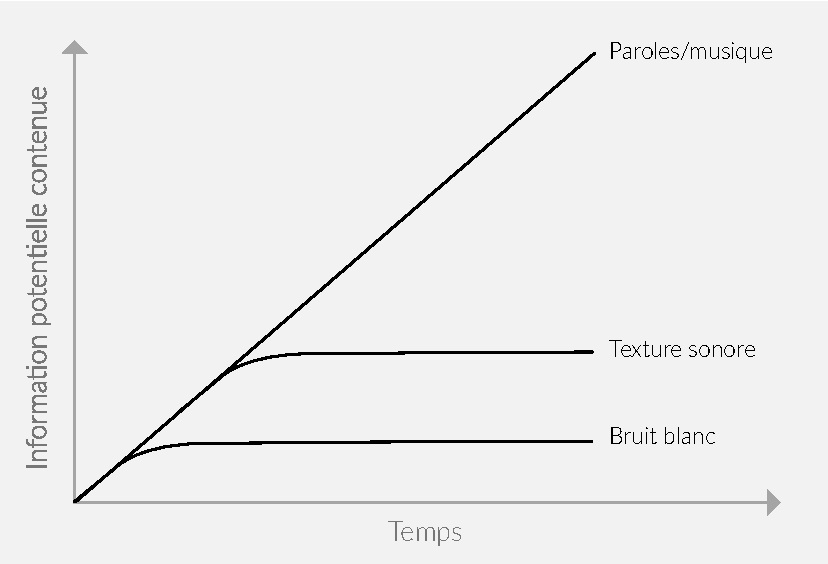
\includegraphics[width=.8\linewidth]{gfx/texture}
        \caption[Information potentielle contenue dans les séquences d'événements, les textures, et le bruit]{Information potentielle contenue dans les séquences d'événements, les textures, et le bruit. D'après \citep{saint1995classification}}\label{fig:texture}
\end{figure}

\subsection{Percevoir les textures}

Contrairement aux événements sonores, la texture est un objet simple, dont le traitement cognitif ne requiert pas une analyse poussée. 

Cela a été mis en évidence par Josh H. McDermott et ses-co auteurs \citep{mcdermott2011sound,mcdermott2013summary}. S'inspirant du fonctionnement de l'oreille humaine, et notamment des processus auditifs intervenant depuis la cochlée, jusqu'au thalamus, \gl{ils ont pu établir un modèle permettant de re-synthétiser} des textures sonores en ne se servant que de statistiques simples, calculées à partir de représentations temps-fréquence de signaux de textures enregistrés. 

Dans une première expérience \citep{mcdermott2011sound}, la capacité des sujets à identifier les textures synthétisées a été testée . Les résultats ont montré que les sons de synthèse étaient aussi bien identifiés que les sons enregistrés. McDermott démontre ainsi qu'une information résumée sous la forme de statistiques, est utile, d'un point de vu cognitif, à la reconnaissance. Dans le cas des textures, ces statistiques constituent même l'unique information disponible, le cerveau ayant fait fi de toute autre représentation plus détaillée \citep{nelken2013ear}.

Dans une seconde expérience \citep{mcdermott2013summary}, les sujets ont du reconnaître, parmi une triade de sons synthétisés, celui produit par une source différente (\ie un type de texture différent, \Cf~Figure~\ref{fig:textureMcder}). Les résultats ont montré que la capacité de discrimination est fonction de la durée des textures. Plus cette dernière est élevée, plus la capacité à discriminer est importante. Ce constat valide les hypothèses formulées par \citep{saint1995classification} sur l'existence d'une période d'attention, nécessaire au cerveau afin de percevoir le stimuli comme une texture. Ces résultats ont aussi montré que le processus de traitement de l'information sonore comprend une prise de décision quant à la nature des stimuli, décision qui va  ensuite influer sur la manière d'analyser l'information montante. L'expérience prouve que cette prise de décision n'a rien d'anodine, car, dans le cas où le cerveau perçoit une texture, il décide sciemment de dégrader l'information, en la résumant de manière statique.

Le fait qu'un jugement perceptif s'améliore avec la durée des stimuli est un principe bien connu en perception des sons\citep{moore1973frequency}. Une troisième expérience de \citep{mcdermott2013summary} a montré cependant que cette vérité n'était pas toujours vérifiée. Au cours de cette expérience, les sujets, soumis à trois exemplaires d'un même type de texture (\eg~trois sons synthétisés de pluie), dont deux étaient produits à partir des mêmes statistiques extraites, ont du identifier le troisième, issu de statistiques différentes (Figure~\ref{fig:textureMcder}). Les résultats ont montré que la capacité des sujets à discriminer le bon stimulus décroît avec la durée des stimuli. Ce fait, qui peut sembler paradoxal, est une conséquence directe du choix du cerveau de ne traiter les textures que sur la base de statistiques. Partant du principe que le signal sonore est analysé suivant des fenêtres d'intégrations successives \citep{yabe1998temporal,poeppel2003analysis}, plus les stimuli sont longs, plus le cerveau est confiant dans le fait qu'il a à faire à des textures, et plus il tend à conserver une information réduite. La réduction de cette information finit éventuellement par gommer les différences fines qui existent entre les stimuli, ce qui ne permet plus de faire la distinction entre eux.


\begin{figure}[t]
        \myfloatalign
        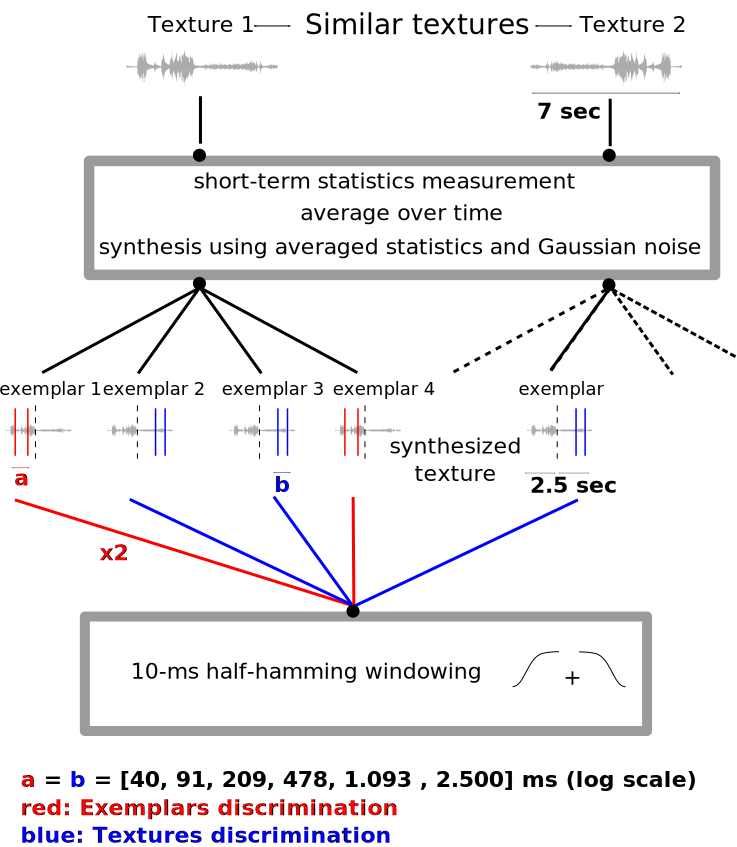
\includegraphics[width=.8\linewidth]{gfx/mcder}
        \caption[Plannification expérientale de l'expérience de discrimination de textures sonores et d'exemplaires de textures sonores]{Plannification expérientale de l'expérience de discrimination de textures sonores et d'exemplaires de textures sonores, menée par \citep{mcdermott2013summary}}\label{fig:textureMcder}
\end{figure}

Une des avancés majeures de ces études est qu'elles apportent de nouvelles réponses sur la nature des représentations sonores stockées en mémoire. Dans le cas des textures, il s'agirait ainsi de descripteurs bas-niveaux, résumés sous la forme de statistiques simples. Cette découverte fait sens d'un point de vue écologique, car elle respecte le principe d'économie de moyens. Le cerveau, reconnaissant que les caractéristiques des textures n'évoluent pas au cours du temps, ne conserve en mémoire qu'une information condensée, qui lui permet pourtant de traiter des sons potentiellement longs. 

Il a été montré que le cerveau peut stocker bien plus que des statistiques. \citep{agus2010rapid} a mis en évidence qu'un bruit blanc, écouté de manière répétée, pouvait être reconnu encore plusieurs semaines après l'écoute, et ce parmi d'autres bruits blancs. Dans ce cas le cerveau emmagasine bien la totalité du signal acoustique.

\subsection{Période d'attention}

\begin{figure}[t]
        \myfloatalign
        \subfloat[]
        {
\includegraphics[width=.5\linewidth]{gfx/xpTexture1}\label{fig:xptexturea}}
        \subfloat[]
        {\includegraphics[width=.5\linewidth]{gfx/xpTexture3}\label{fig:xptextureb}}
        \caption[Événement ou texture sonore: influence de la période d'attention]{Événement ou texture sonore: influence de la période d'attention. (a) la nature des stimuli utilisés. (b) le seuil d'espacement moyen permettant de faire la distinction entre une séquence d'événements et une texture}\label{fig:xptexture}
\end{figure}

Nos travaux ont également porté sur cette notion de période d'attention. Comme nous l'avons vu, la texture est un objet composite. En poussant cette vision à l’extrême, une texture peut être vue comme un empilement d’événements sonores, ayant cessés d'être perçus de manière distincte, dès lors qu'ils forment un tout homogène et stable. 

Nous avons suivi cette idée, afin de bâtir un protocole permettant d'analyser la période d'attention. En considérant comme stimuli une mixture d'événements du même type, nous faisons l'hypothèse qu'à partir du moment où le cerveau parvient à isoler un événement de cette mixture, il ne perçoit plus la mixture comme une texture, mais comme une succession d'événements. Inversement, s'il ne parvient pas à distinguer un événement isolé, alors la mixture est perçue comme une texture.

Sur la base de cette hypothèse, une expérience de reconnaissance de type oui/non (\Cf~Annexe~\ref{app:xp_texture} pour une description exhaustive de l'expérience) a été montée. Dans cette expérience, chaque stimuli est composé d'un son cible, suivi d'une séquence d'événements enchevêtrés. Tous les événements sont des sons isolés ayant une durée de $1$ seconde. La séquence dure 6 secondes (\Cf~\ref{fig:xptexturea}). L'objectif pour le sujet est d'indiquer si oui ou non il a entendu le son cible dans la séquence d’événements.

Les séquences donnent à entendre des scènes de trafic. Ces scènes sont simulées en agglomérant des sons de voiture isolés. La simulation est contrôlée par un paramètre réglant l'espacement temporel inter-onset moyen entre les événements. Cinq valeurs d'espacement sont considérées: $0.1$, $0.3$, $0.5$, $0.7$ et $0.9$ secondes. Pour chaque espacement, nous simulons 20 séquences de trafics, chaque sujet devant alors écouter 100 stimuli. La moitié de ces stimuli sont des pièges, le son cible y étant absent. Nous mesurons les performances des sujets en utilisant la mesure de sensitivité $d'$ (\Cf~Annexe~\ref{app:sdt}). Les résultats sont très encourageants. Ils montrent qu'il existe bien un espacement limite à partir duquel la mixture cesse d'être perçue comme une texture. Pour des sons isolés d'une seconde, cet espacement limite est de 0.42 secondes, soit la moitié de la durée des événements utilisés (\Cf~Figure~\ref{fig:xptextureb}).






%*****************************************
%*****************************************
%*****************************************
%*****************************************
%*****************************************
